% !TEX root = ../main.tex

\chapter{词嵌入模型}

近些年,作为机器学习最重要的一个分支,深度学习成为科研人员关注的热点问题,并且深度学习模型在计算机视觉、自然语言处理、语音识别、数据挖掘等领域发挥了至关重要的作用。深度学习模型通过使机器模仿人类的感官和思想方式,挖掘大量的、多维度数据背后的潜在规则,解决了很多复杂的模式识别疑难问题,为人类迈向人工智能做出了突出贡献。不仅仅在上述领域,如今在生物信息学和基因组学方面,深度学习也带来了巨大的改变。在大数据时代,深度学习通过将生物医学大数据转化为有价值的领域知识极大简化了蛋白质功能研究和药物发现研究的历程。

传统的机器学习方法在研究的过程中,科研人员需要利用特征工程手动在原始序列数据的领域知识上提取特征,然后再部署相关的机器学习算法,这样的做法比较耗时而且极大的依赖于生物信息学和基因组学的专业知识。随着深度神经网络的兴起,传统的特征提取方法已经在很大程度上被序列编码方法,即词嵌入表征学习所取代。深度学习模型通过将组成生物序列的单词编码成稠密、连续的低维向量获得比离散特征提取表示更好的性能。由于在 NLP 领域的词向量和深度学习技术已经趋于成熟,同时生物序列和文本序列具有一定的相似性,可以通过将 NLP 中的词嵌入方法和深度学习模型迁移到生物信息学进行深入研究和探索。本章将重点介绍 NLP 领域中的词嵌入方法。

\section{基于神经网络的词嵌入方法}
词嵌入(Word Embedding)是一种将文本中的单词转化为稠密数字向量的方法。为了使计算机能够识别输入的特征,就需要把这些被转换成数字的向量以数字形式作为输入使用深度学习模型进行分析。

早期的词嵌入方法通常采用独热编码(One-hot)的方式,它使用一个词汇表大小的向量来表示文本中的词,其中只有对应于该词的项是1而所有其他的项都是零。One-hot 编码的最大问题在于不能表示词与词之间的相似性。我们通过点积计算向量之间的相似性。在One-hot编码中,语料库中任何两个词之间的点积总是为零,即任意两个词是正交的。随着深度学习的兴起,基于深度学习的词嵌入方法能够在没有任何人的干预下自主学习单词的潜在语义,同时可以表示词与词之间的相似性。我们不需要计算和存储关于某个庞大的数据集(可能是数十亿个句子)的全局信息,我们可以尝试创建一个模型,该模型将能够一次学习一个迭代,并最终能够根据上下文对单词的概率进行编码。其思想是设计一个以词向量为参数的模型。然后,针对特定的目标函数对模型进行训练。在每次迭代中,我们运行通过运行模型计算误差,并遵循相应的参数更新规则,该规则可以对导致误差的错误进行惩罚。通过这种机制,我们学习到了模型的词嵌入表征。目前,基于深度学习的词嵌入方法已经广泛应用于 NLP 领域的各种任务中,例如文本分类,情感分析,机器翻译等等。

蛋白质序列同自然语言处理中的文本一样,由很多单词排列组合构成。蛋白质序列由20几种连续的氨基酸构成,是研究蛋白质功能的基础。我们可以将组成蛋白质序列的氨基酸类比于组成文本的单词,将蛋白质序列信息类比于文本中句子的语义信息。因此,NLP 领域中的词嵌入方法非常适合于蛋白质序列领域的研究,下面将介绍4种本文用到的词嵌入方法。

\subsection{Word2Vec}
Word2Vec \cite{mikolov2013distributed} 词嵌入表征是由 Mikolov 等人于 2013 年提出的一种词嵌入方法。它包含两个学习模型,分别是 continuous bag-of-words (CBOW) 和 skip-gram. CBOW 旨在根据词向量从上下文信息中预测中心词,skip-gram则做了相反的事情,它从中心词预测上下文单词的分布(概率)。

\begin{figure}[!htp]
\centering
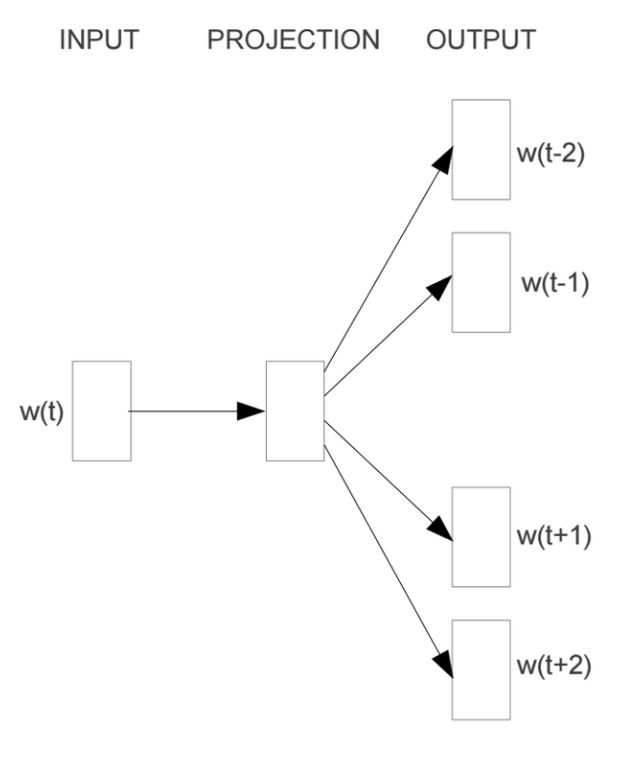
\includegraphics[width=0.6\textwidth]  {imgs/skip-gram.png} \\
\bicaption[Skip-gram\cite{mikolov2013distributed}图示]
    {Skip-gram\cite{mikolov2013distributed}图示。}
    {Model architecure of Skip-gram\cite{mikolov2013distributed}.}
\label{fig:skip-gram}
\end{figure}

这里我们以 skip-gram 模型为例详细的介绍。如图 \ref{fig:skip-gram} 所示,我们假设上下文的窗口为$2m$,即以中心词为中心,分别向左和向右选取$m$个单词,那么给定中心词预测上下文单词的概率为:

\begin{equation}
    P(\omega_c|\omega_o) = \frac{exp(u_o^{T} v_c)}{\sum_{i \in V} exp(u_i^{T} v_c)}
\tag{3-1}
\end{equation}
其中 $\omega_o$ 和 $\omega_c$ 分别代表中心词和上下文单词,$u_o$和$u_c$分别代表中心词向量和上下文词向量,$V$是全体词汇表。这个概率就是给定中心词的条件下,某个词是上下文词的概率。这里假设在给定中心词的条件下每个单词出现的概率是独立的,类似朴素贝叶斯的条件独立性假设,可以大大的简化运算,将上式改写为连乘的形式如下:

\begin{equation}
   \prod \limits_{t=1}^T \prod \limits_{-m\leq j \leq m, j \neq 0} P(\omega^{(t+j)}|\omega^{(t)})
\tag{3-2}
\end{equation}
其中$t$表示中心词的位置,$m$为窗口大小,这样就得到了每个中心词的计算上下文词的概率。在该公式中变量是上下文词向量和中心词向量,于是只要改变参数使得目标最大化就可以。这里使用极大似然估计,对上式取负对数得到:

\begin{equation}
   -\sum \limits_{t=1}^T \sum \limits_{-m\leq j \leq m, j \neq 0} log^{P(\omega^{(t+j)}|\omega^{(t)})}
\tag{3-3}
\end{equation}

对上式进行参数求导可以计算梯度,更新参数。梯度下降优化结束后,我们便能得到两个向量 $u$ 和 $v$,分别表示上下文词向量和中心词向量,这就是我们要找的词向量。

Word2Vec作为预训练的词嵌入方法,通常语料库包含上千万条数据,词汇表中的单词数量通常有上万个,因此在目标函数中计算所有单词的softmax概率需要消耗巨大的计算资源。对此,Mikolov等人提出了负采样和层级softmax方法简化模型的复杂度和参数量。

负采样的思想为,对于每个训练步骤,我们可以只采样几个反例而不是计算整个词汇表。层级 softmax 使用二叉树来表示词汇表中的所有单词。二叉树的每一个叶子节点都表示一个单词,从根节点到叶子节点都有一条独特的路径。一个单词作为输出词的概率表示为从根节点随机游走到该词叶节点的概率。计算成本从 $O(V)$ 降低为 $O(log^{V})$。

Daniel 和 David 等人 \cite{buchan2019inferring} 使用 Word2Vec 证明了蛋白质域在多域蛋白质的上下文中可能具有语义意义。在这项工作中,他们将多域蛋白质视为文本中的句子,其中域标识符视为句子中划分的单词。 通过使用 Interpro \cite{finn2017interpro} 真核蛋白质作为语料库,他们证明了 Word2Vec 可以获得具有功能意义的蛋白质域嵌入。


\subsection{GloVe}
Word2Vec 模型通过在上下文窗口中进行预测来学习单词嵌入,该模型具有捕获单词相似性的复杂语言模式的能力,但是未能利用全局共现统计。GloVe \cite{pennington2014glove} 是由 Pennington 等人于2014年提出的基于单词共现统计的词嵌入方法。相比之下,GloVe 由一个加权最小二乘模型组成,该模型在全局单词-单词间共现概率矩阵上进行训练,从而有效地利用了统计数据。 该模型生成了一个具有有意义子结构的词向量空间。它在单词类比任务上显示了最先进的性能,并且在几个单词相似性任务上优于其他的方法。

首先定义词与词之间的共现矩阵为 $X$,其中 $X_{ij}$ 是语料库中出现在单词 $i$ 上下文中单词 $j$ 的次数。定义 $X_i = \sum_{k} X_{ik}$ 表示单词 $i$ 的上下文所有单词的总个数。最终 $P_{ij} = P(j|i) = \frac{X_{ij}}{X_i}$ 表示单词 $j$ 出现在单词 $i$ 上下文的概率。

\begin{table}[!htbp]
\centering
\bicaption[GloVe \cite{pennington2014glove} 中共现矩阵示例]{GloVe \cite{pennington2014glove} 中共现矩阵示例。}{Example of GloVe \cite{pennington2014glove} co-occurrence matrix.}
\scalebox{1.25}{
\begin{tabular}{c|c|c|c|c}
\hline
概率和比率 & k=solid & k=gas & k=water & k=fashion\\
\hline
$P(k|ice)$ & $1.9\times10^{-4}$ & $6.6\times10^{-5}$ & $3.0\times10^{-3}$ & $1.7\times10^{-5}$\\
\hline
$P(k|stream)$ & $2.2\times10^{-5}$ & $7.8\times10^{-4}$ & $2.2\times10^{-3}$ & $1.8\times10^{-5}$\\
\hline
$P(k|ice)/p(k|stream)$ & 8.9 & $8.5\times10^{-2}$ & 1.36 & 0.96\\
\hline
\end{tabular}}
\label{tabel:glove-1}
\end{table}

表\ref{tabel:glove-1}表明,单词的词向量应该和单词共现概率的比率有关,而不是他们的概率本身。由表\ref{tabel:glove-1}看出 $P(i|k)/P(j|k)$ 的取值是有一定规律的,定义函数 $F(w_i,w_j,w_k) = P(i|k)/P(j|k)$, Pennington 等人对共现概率的比率进行了总结如表 \ref{table:glove-2} 所示:

\begin{table}[!htbp]
\centering
\bicaption[GloVe \cite{pennington2014glove} 中共现概率比率的规律。]{GloVe \cite{pennington2014glove} 中共现概率比率的规律。}{The law of GloVe \cite{pennington2014glove} co-occurrence probability ratio.}
\scalebox{1.2}{
\begin{tabular}{c|c|c}
\hline
$F(w_i,w_j,w_k)$ & 单词j,k相关 & 单词j,k不相关 \\
\hline
单词i,k相关 & 趋近于1 & 很大 \\
\hline
单词i,k不相关 & 很小 & 趋近于1\\
\hline
\end{tabular}}
\label{table:glove-2}
\end{table}

GloVe经过推理,定义目标函数(损失函数)如下:

\begin{equation}
  J = \sum \limits_{ik} f(X_{ik}){(w_i^{T}w_k + b_i + b_k - log(X_{ik}))}^2
\tag{3-4}
\end{equation}
其中$X_{ik}$表示单词$i$和$j$的共现次数,$f(X_{ik})$ 表示共现次数的权重因子,$f(x)$的定义如下:

\begin{equation}
 f(x) = \left\{
    \begin{array}{lr}
    (\dfrac{x}{x_{max}})^\alpha, & if x < x_{max} \\
    1, & otherwise\\
    \end{array}
\right.
\tag{3-5}
\end{equation}

函数$f(x)$有三个特点:(1)$f(0) = 0$,即两个单词没有共同出现过,权重为0;(2) $f(x)$是非减函数,如果两个单词共同出现的次数多,权重反而变小了,这违反了设置权重因子的初衷;(3)$f(x)$对于较大的$x$不能取太大的值,因为出现频率过高的词通常是一些无意义的单词。通过以上公式,可以将权重因子$f(x)$设置在一个合理的范围之内。根据经验,Pennington 等人任务 $x_{max} = 100, \alpha = \frac{3}{4}$ 是一个比较好的选择。 

综上所述,GloVe 模型通过对单词-单词共现矩阵中的非零元素进行训练来有效地利用全局统计信息,并生成具有有意义的子结构的向量空间。目前蛋白质的研究领域还没有使用 GloVe 词嵌入方法的研究成果。

\subsection{FastText}

FastText \cite{joulin2016bag} 是由 Facebook AI Research 开源的一个文本分类器,用于有效的学习单词嵌入表示和句子分类类别。模型拥有快捷的训练速度,适合在大型数据集上进行训练。相比于其他的文本分类模型,例如 SVM,逻辑回归,神经网络等,FastText 可以在保证分类准确率的情况下,大大的降低训练时间。


\begin{figure}[!htp]
\centering
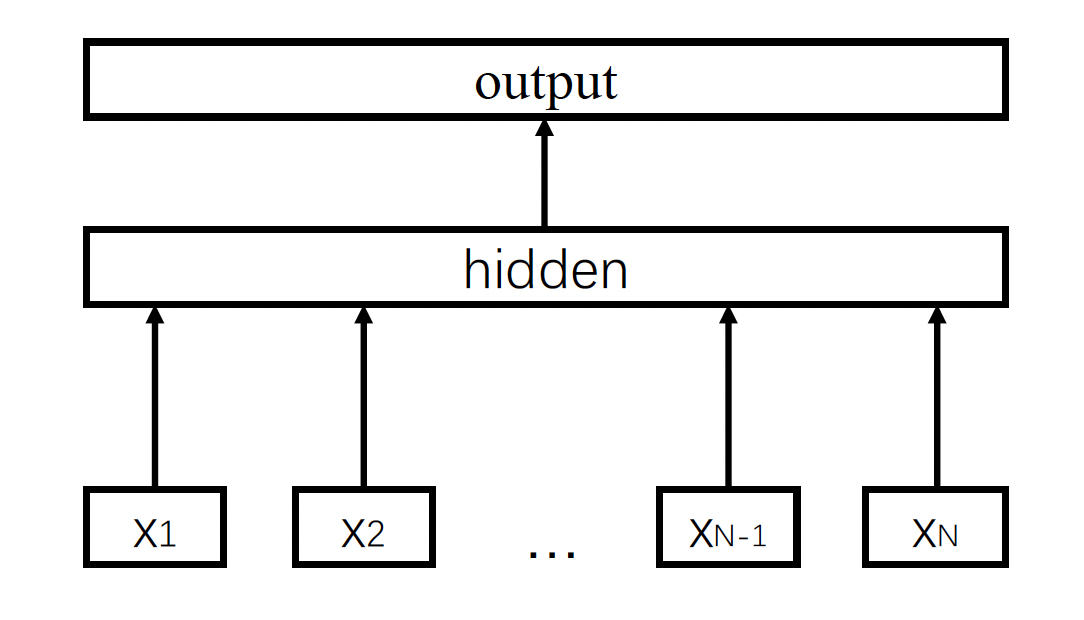
\includegraphics[width=0.9\textwidth]  {imgs/fasttext.png} \\
\bicaption[FastText \cite{joulin2016bag} 图示]
    {FastText \cite{joulin2016bag} 图示。}
    {Model architecure of FastText \cite{joulin2016bag}.}
\label{fig:fasttext}
\end{figure}

图\ref{fig:fasttext}为 FastText 的结构图。FastText 模型输入一个序列(可以是一句话,也可以是一段文本),输出这个序列在各个文本类别上的概率分布。FastText 模型结构和 Word2Vec 中的 CBOW 结构很相似,一共有三层,分别是输入层、隐藏层和输出层。首先将输入的序列划分为单词的特征向量,经过线性变换映射到隐藏层进行叠加求平均操作,最终线性变换映射到文本的类别标签。FastText 和 Word2Vec 的不同之处在于,在 Word2Vec 中将每一个单词视为要找到整个序列向量表示的最小单位;但在 FastText 中,采用 n-gram 对单词进行切分,即一个单词由 n-gram 个字符组成。为了加速训练的速度,FastText 中也采用了层级 softmax ,利用了类别分布不均衡的优势,通过使用哈夫曼编码建立基于类别表征的二叉树。因此,FastText 的核心工作是将构成序列的单词以及 n-gram 向量进行叠加平均操作得到序列向量,然后使用序列向量进行 softmax 多分类任务。

综上所述,FastText 使用一个浅层的神经网络能够达到媲美深度神经网络的分类精度,并且拥有高效的训练速度。可以在不使用 GPU 的情况下,利用 CPU 完成词嵌入向量的训练。Le 和 Huynh 等人\cite{le2019identifying} 结合 FastText 架构和氨基酸的嵌入表征来识别 SNARE。他们任务可以将 FastText 模型应用于生物信息学,可以为蛋白质测序预测提供基础。本文基于 FastText 模型结构构建了一个分类模型,可以同时用于蛋白质序列的嵌入表征学习以及蛋白质序列的分类任务。

\subsection{Doc2Vec}
Le 和 Mikolov 等人于 2014 年提出的 Doc2Vec 模型 \cite{le2014distributed} 是对 Word2Vec 模型的扩展。虽然 Word2Vec 可以提高比较准确的词向量,在一些任务中表现优异,但是还不存在一个有效的模型将它们结合成一个序列或者文档向量,因此 Doc2Vec 主要是对较大的文本块(例如段落或者整个文档等)的连续嵌入表示进行无监督学习。

和 Word2Vec 相似,Doc2Vec 也包含两个学习模型,一种是分布记忆的段落向量(PV-DM),类似于 Word2Vec 中的 CBOW 模型;另一种是分布词袋的段落向量(PV-DBOW),类似于 Word2Vec 中的 skip-gram 模型。
Doc2Vec 的训练过程和 Word2Vec 基本一致,每次迭代从一段话中利用滑动窗口采样固定长度的单词序列,其中的一个单词作为输出的预测词,其他单词作为输入词。不同之处在于,Doc2Vec 在 Word2Vec 的基础上增加了句子向量,同词向量一起作为输入层的输入,之后将所有的向量叠加求平均生成一个新的隐藏向量,进而使用这个隐藏向量预测滑动窗口内的预测词。句子向量在同一段文本的若干次滑动窗口迭代训练中是共享的,可以看作是该句子的主旨,因此拥有记忆功能,弥补了 Word2Vec 中忽略了本次窗口中训练的词以外文本中的其他词的不足。

Yang \cite{yang2018learned} 等人利用 Word2Vec 和 Doc2Vec 两种模型学习蛋白质的嵌入表征,由于蛋白质序列的长度相比普通的文本句子要长很多,因此 Doc2Vec 非常适合大文本的蛋白质序列嵌入表征学习。本文利用了 Doc2Vec 的 PV-DM 模型作为预训练任务学习蛋白质序列的嵌入表征。



